\documentclass[xcolor=dvipsnames]{beamer}
\usepackage{hyperref}
\usepackage[utf8]{inputenc}
\usepackage[ngerman]{babel}
\usepackage{multicol}
\usepackage{graphicx}

% appearance
\usetheme{Boadilla}
\usecolortheme[named=Black]{structure}
\setbeamertemplate{navigation symbols}{}%remove navigation symbols

\hypersetup{
	colorlinks=true,
	linkcolor=white,
	urlcolor=blue,
	citecolor=black
}

% content
\title{Sichere E-Mails mit PGP}
\author{Peter Gewald \& Manuel Groß}
\date{2015-11-15}

\begin{document}
\titlepage
\hfill\scalebox{.6}{\href{http://creativecommons.org/licenses/by-sa/3.0}{CC-BY-SA 3.0}}

\frame{
	\frametitle{Wer sind wir?}
	\center{
		\begin{multicols}{2}
			
\includegraphics[scale=0.4]{images/ccc-ol-black}\\[0.1cm]
			\url{https://ccc-ol.de/}\\
			\columnbreak
			\ \\[0.5cm]
			
\includegraphics[scale=0.38]{images/mainframe_logo}\\[0.1cm]
			\url{https://mainframe.io/}
		\end{multicols}
	}
}

\frame{
	\frametitle{Was ist eigentlich unser Problem?}
	\center{
		
\includegraphics[scale=0.2]{images/-FsA14_-_Freiheit_statt_Angst_027_(14898399419)_(2)}\\
		\scalebox{.6}{\href{https://creativecommons.org/licenses/by-sa/2.0/deed.en}{CC-BY-SA 2.0} \href{https://commons.wikimedia.org/wiki/File:-FsA14_-_Freiheit_statt_Angst_027_(14898399419)_(2).jpg}{Markus Winkler}}\\[0.2cm]\pause
		\begin{itemize}
			\setlength\itemsep{0em}
			\item \href{https://de.wikipedia.org/wiki/Globale_\%C3\%9Cberwachungs-_und_Spionageaff\%C3\%A4re}{Massenhafte, anlasslose Überwachung}\pause
			\item \href{https://de.wikipedia.org/wiki/Andrej\_Holm\#Ermittlungsverfahren\_wegen\_Verdachts\_der\_Mitgliedschaft\_in\_einer\_terroristischen\_Vereinigung}{False Positives}\pause 
			\item \href{http://www.netzpiloten.de/der-chilling-effect-massenueberwachung-zeigt-soziale-folgen/}{Chilling Effect}
		\end{itemize}
	}
}

\frame{
	\frametitle{Lösungsvorschlag: Verschlüsselung}
	\begin{itemize}
		\setlength\itemsep{0em}
		\item wandelt Klartext in unlesbares Kauderwelsch um
		\item kann mit Kenntnis über Verschlüsselung und dem Schlüssel umgekehrt werden
		\item üblicherweise ein mathematisches Verfahren mit geheimem Eingabewert
	\end{itemize}\pause
	\begin{itemize}
		\item symmetrisch
		\begin{itemize}
			\item ver- und entschlüsseln mit selbem Schlüssel und selben Verfahren
		\end{itemize}
	\end{itemize}\pause
	\begin{itemize}
		\item asymmetrisch
		\begin{itemize}
			\item ver- unt entschlüsseln mit unterschiedlichen Schlüsseln und selbem Verfahren
		\end{itemize}
	\end{itemize}
}

\frame{
 	\frametitle{Was wir nicht meinen...}
	\begin{itemize}
		\item Transportwegeverschlüsselung (TLS, ...)
		\item DE-Mail (jemand anderes hat auch einen Key)
	\end{itemize}
}

\frame{
	\frametitle{Asymmetrische Verschlüsselung}
	\begin{center}
		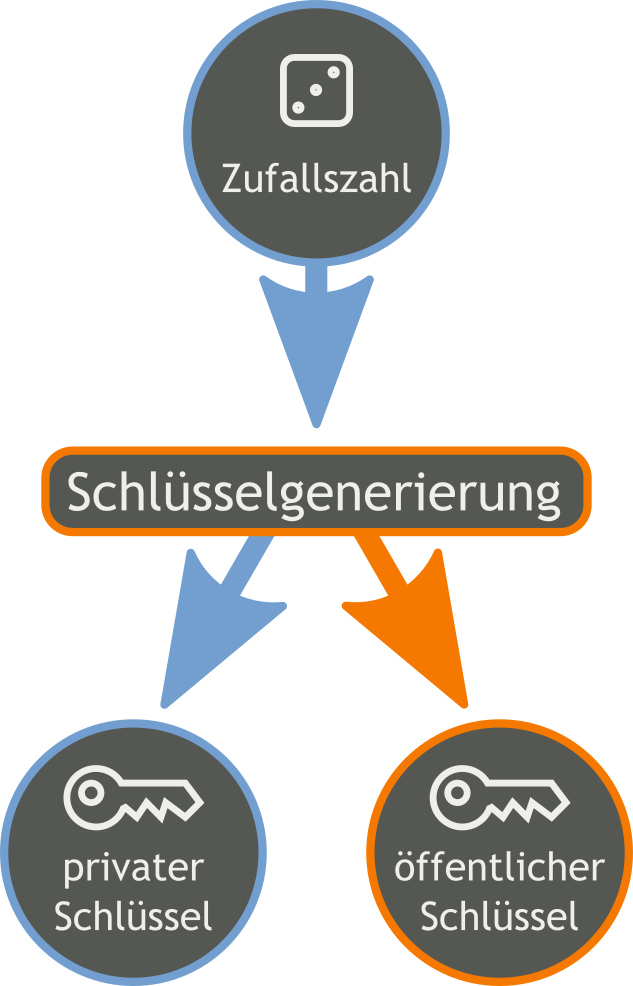
\includegraphics[scale=0.3]{images/Orange_blue_public_private_keygeneration_de}
	\end{center}
}

\frame{
	\frametitle{Asymmetrische Verschlüsselung}
	\begin{center}
		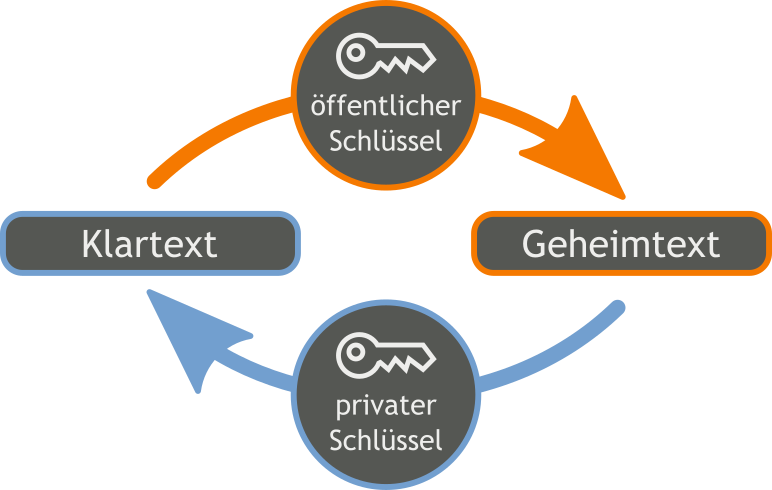
\includegraphics[scale=0.4]{images/Orange_blue_public_key_cryptography_de}\\
	\end{center}
}

\frame{
	\frametitle{Problem: Vertrauenswürdigkeit}
	\begin{block}{Problem:}
		Wer garantiert uns, dass Bob wirklich der Absender ist?
	\end{block}
	\vfill
	\begin{itemize}
		\item Idee: zentraler Ansatz
		\begin{itemize}
			\item Indirekter Austausch über Dritte (z.B. Browser oder Mailprogramm)
			\item Hierarchie/Zertifikatsliste (schonmal reingeschaut?)
		\end{itemize}
	\end{itemize}
	\begin{center}
		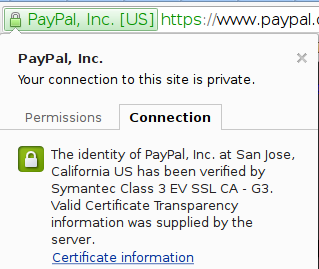
\includegraphics[scale=0.4]{images/paypal_example.png}
	\end{center}
}

\frame{
	\frametitle{Unterschiedliche Ansätze: Verteilt}
	\begin{center}
		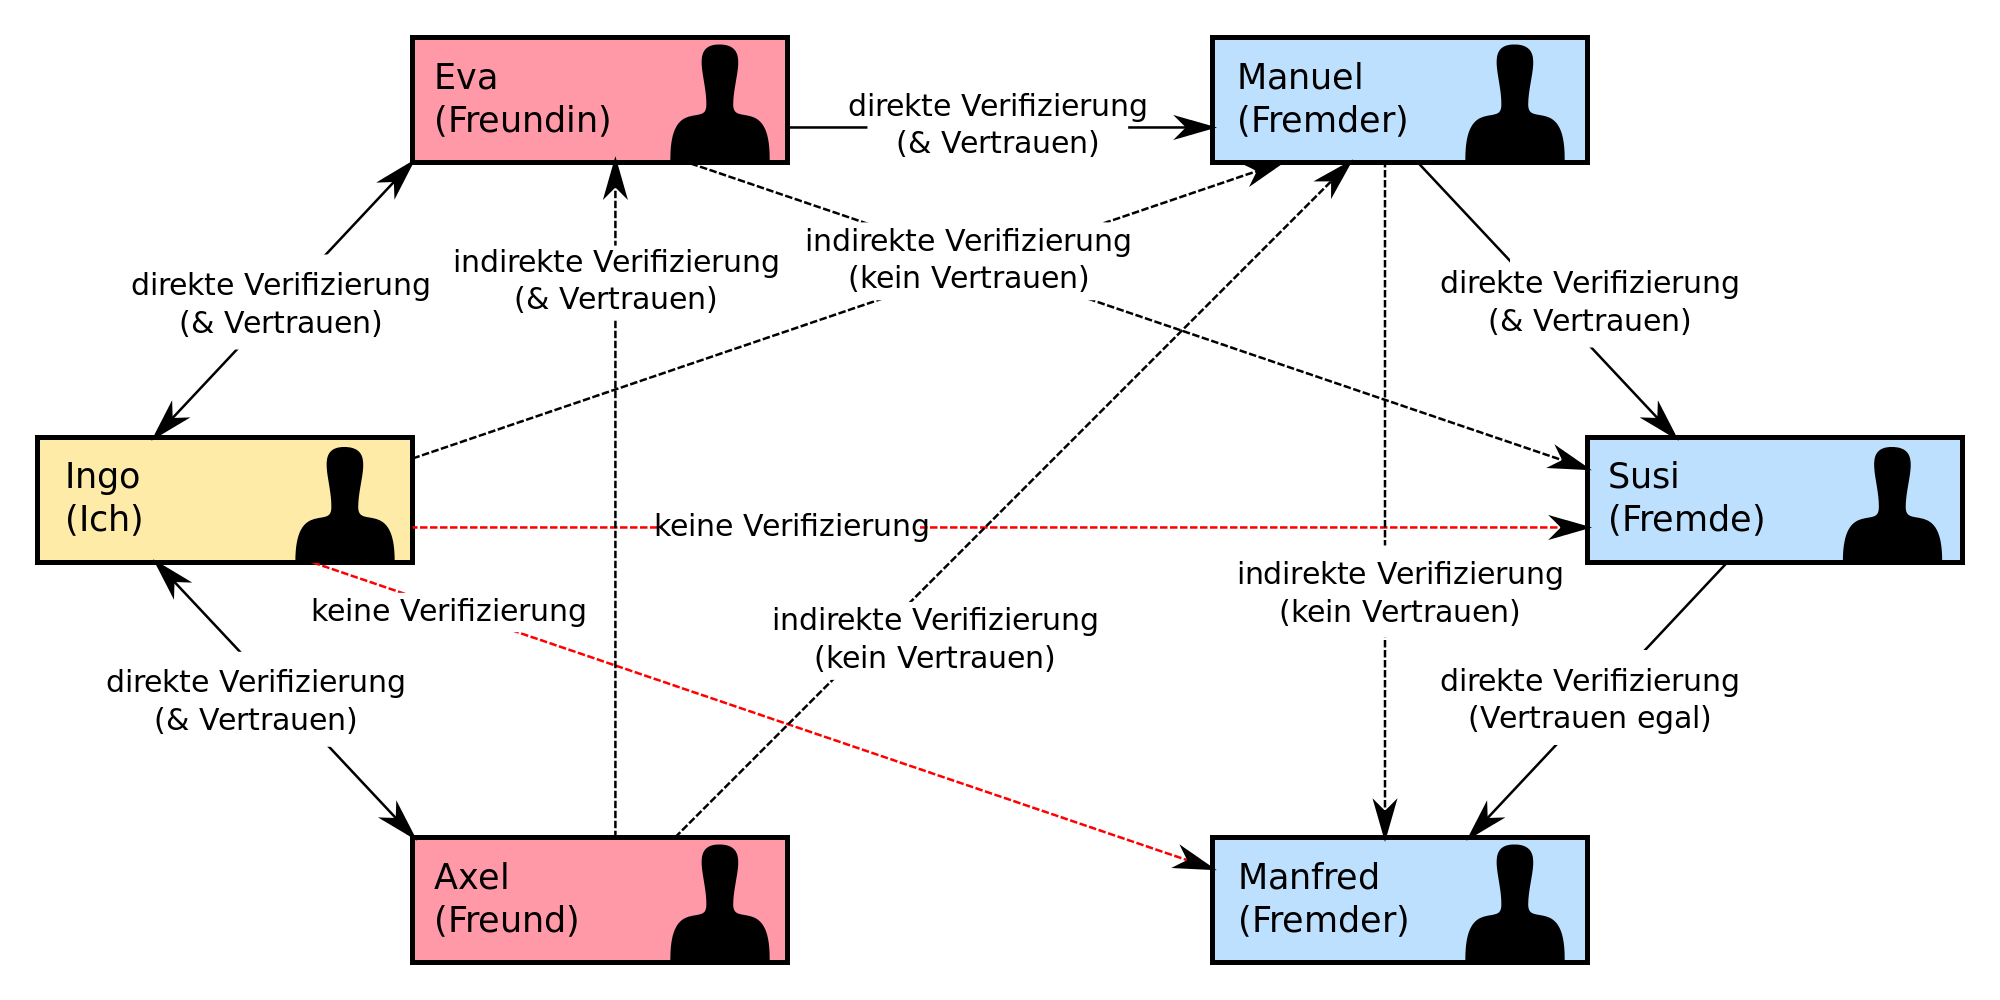
\includegraphics[scale=0.17]{images/Web_of_Trust_2}\\[0.1cm]
		\scalebox{.6}{\href{http://creativecommons.org/licenses/by-sa/3.0}{CC-BY-SA 3.0} \href{https://de.wikipedia.org/wiki/Web_of_Trust\#/media/File:Web_of_Trust_2.svg}{Hauke Laging}}
	\end{center}
}

\frame{
	\frametitle{Cryptoparties}
	\begin{center}
		% TODO: Foto eines Fingerprints machen und einfügen
		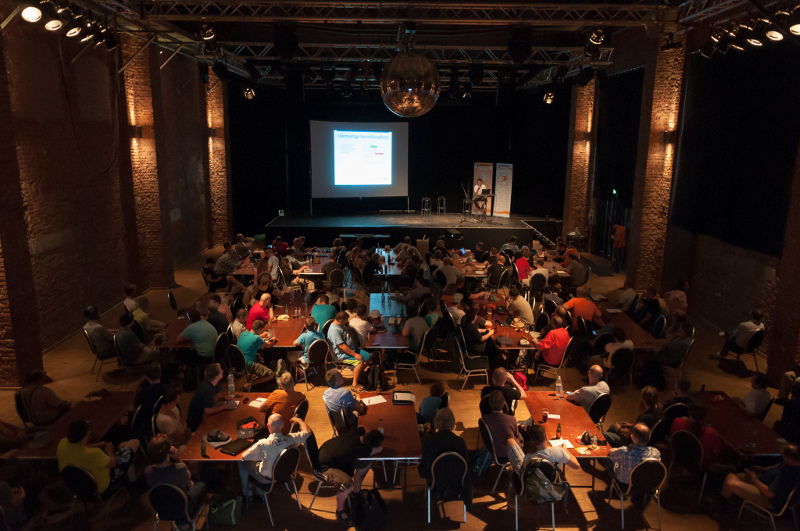
\includegraphics[scale=0.11]{images/9392567326_65566b7a2a_k}\\[0.1cm]
		\scalebox{.6}{\href{https://creativecommons.org/licenses/by/2.0/}{CC-BY 2.0} \href{https://www.flickr.com/photos/67481069@N06/9392567326/in/photolist-dgF9o5-dgFfuU-jfFAJZ-Aahk2f-zfxU6C-zUZu93-derAa9-Aczqq4-zfxQK9-AdxznB-zfxXq3-zV4Y9p-AaheUm-AcztSV-zfxSg5-nRTQw1-AahmXQ-nSfhAn-AahnKw-zUZxHs-Abpgpm-dQPB55-dQPB6U-dQPB5s-zfFUrR-Aczz1a-AdxwMr-Adxwpn-AczwBc-zfFYEF-Adxrqe-AczrPX-zUY3t9-zfFVhP-Abpoh9-f76gGL-dQPB2A-dQPB3m-dgjJfx-AczogV-zUYbys-AdxumK-AdxtAM-jHvNzD-fiZn2Y-edbqzd-fiK8LB-d54cjd-qWi8VV-npuuAT}{wbritzl}}\\\pause
		\begin{itemize}
			\setlength\itemsep{0em}
			\item Neue Leute kennenlernen\pause
			\item Spaß an lustigen, alten, Ausweisbilder anderer haben!\pause
			\item Irgendwas mit Sicherheit\pause
			\item Selbst Cryptoparties veranstalten!
		\end{itemize}
	\end{center}
}

\frame{
 	\frametitle{Signatur}
	,,Nebeneffekt` der Authentizitätsprüfung
	\begin{center}
		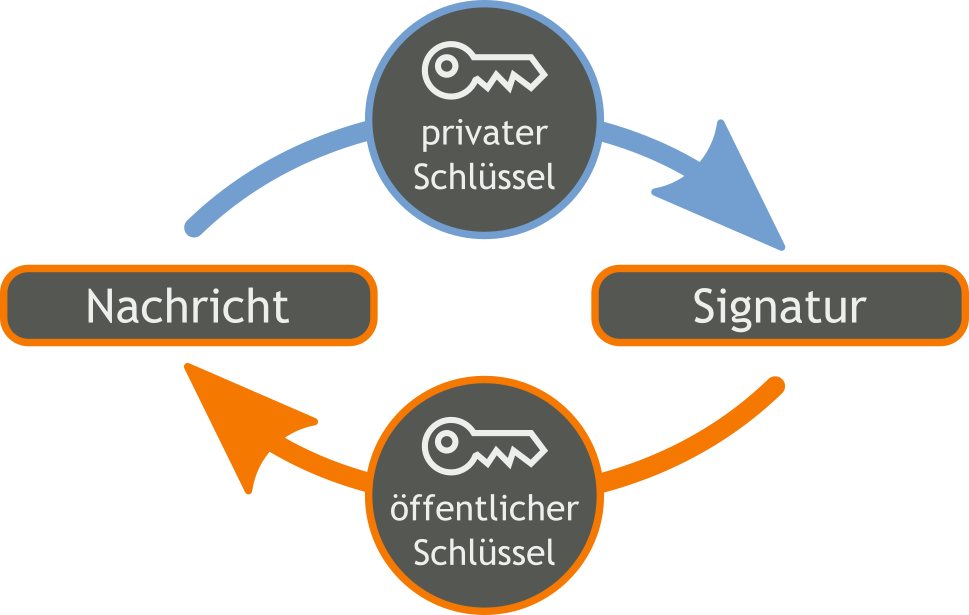
\includegraphics[scale=0.38]{images/Orange_blue_digital_signature_de}
	\end{center}
}

\frame{
	\frametitle{GPG}
	Was ist jetzt eigentlich GPG?
	\begin{center}
		
\includegraphics[scale=0.38]{images/gnuPG.png}\\
		{\tiny \url{https://gnupg.org}}
	\end{center}
	\begin{itemize}
		\item<1-> ,,Gnu Privacy Guard``, Open Source-Implementierung von OpenPGP
		\item<1-> ,,PGP`` (,,Pretty Good Privacy``), alternative, nun proprietäre Implementierung
		\item<1-> Sehr verbreitet im Open Source Umfeld
		\item<2-> Eher ungebräuchlich im geschäftlichen Umfeld
		\item<2-> Web of Trust Prinzip
		\item<3-> Plugins für viele Clients
		\item<3-> Metadaten nicht verschlüsselt!
		\item<3-> Teilweise Probleme mit Wrapping (z.B. \href{https://lwn.net/Articles/584542/}{Thunderbird})
	\end{itemize}
}

\frame{
	\frametitle{PGP funktioniert!}
	\begin{center}
		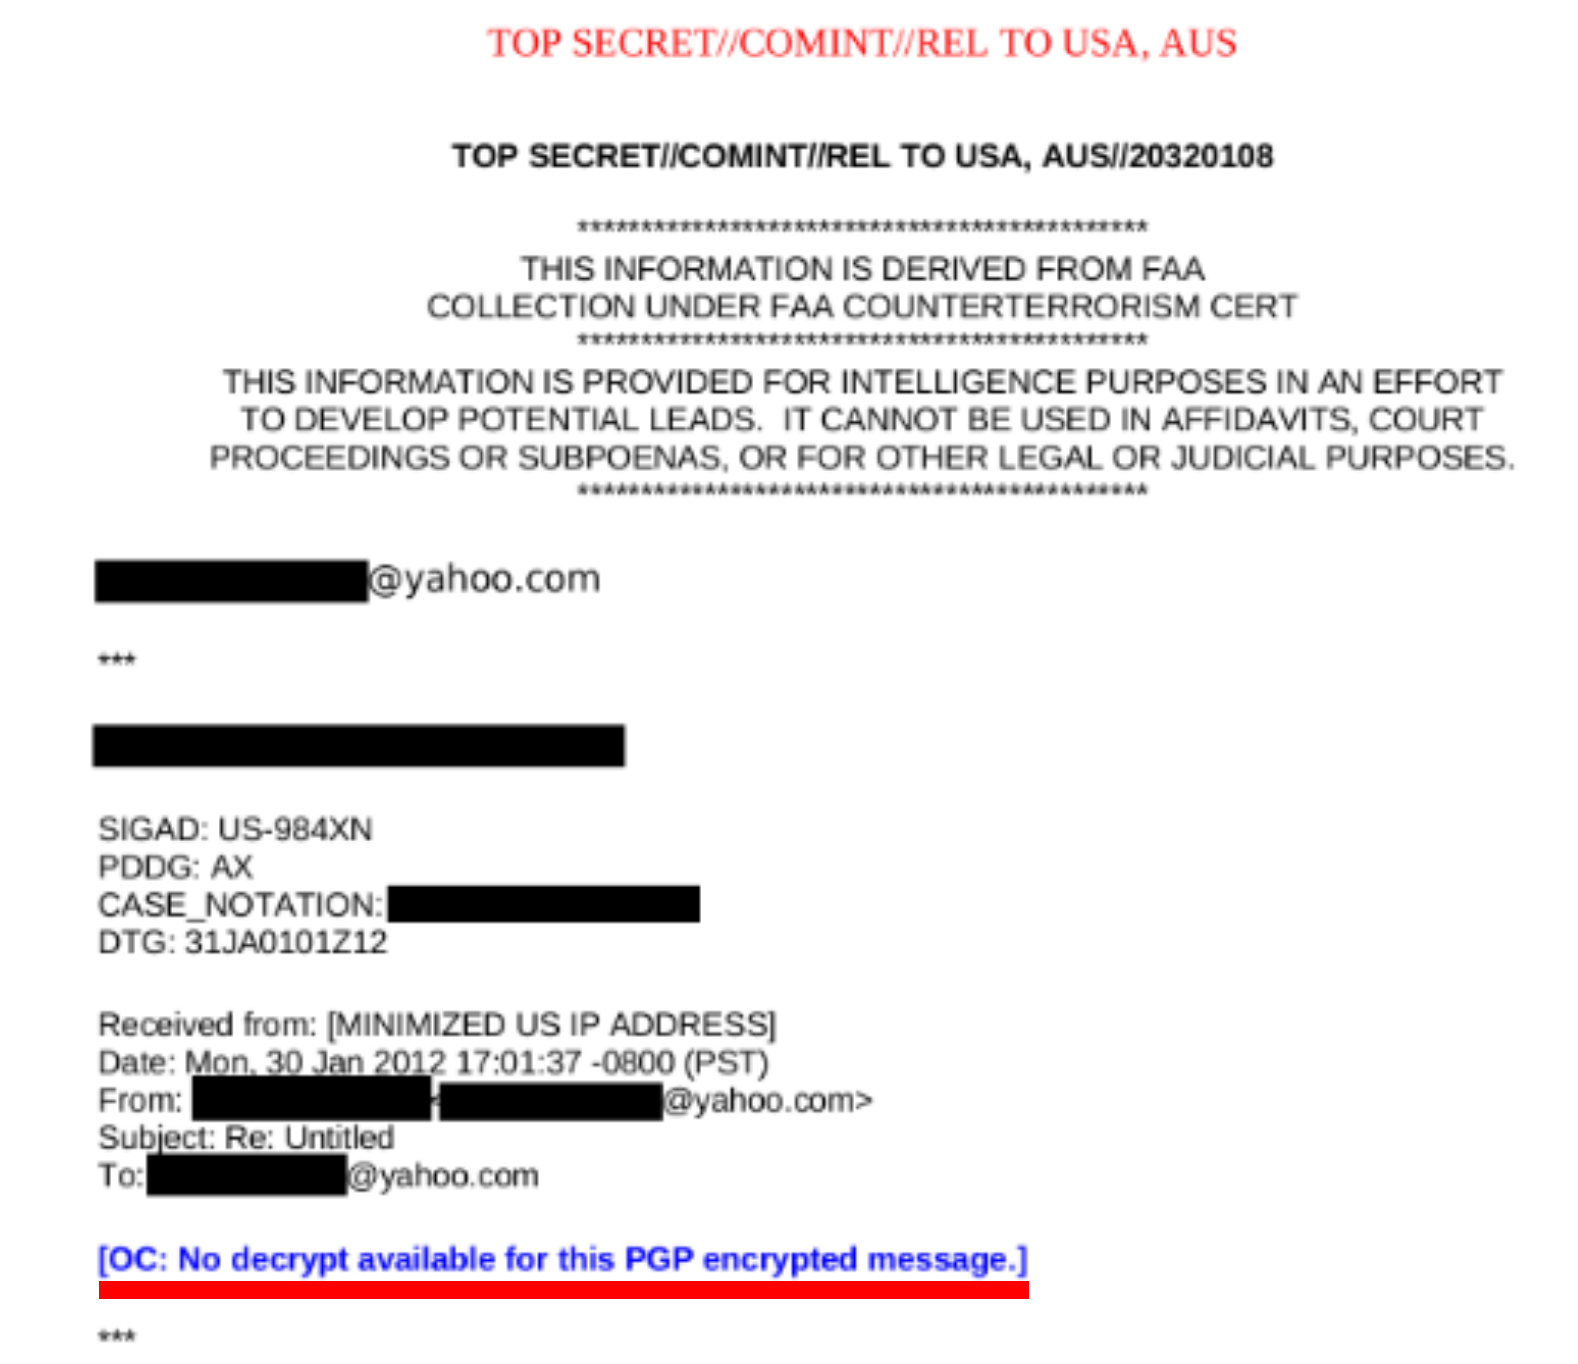
\includegraphics[scale=0.16]{images/snowden}
	\end{center}
}

\frame{
	\frametitle{GPG unter Linux - Installation}
	{\bf Debian Pakete:}
	\begin{itemize}
		\item gnupg2
		\item signing-party (für caff)
		\item msmtp
	\end{itemize}
}

\frame{
	\frametitle{GPG unter Linux - Konfiguration}
	\begin{itemize}
		\item Config: $\sim$/.gnupg/gpg.conf
		\item {\tt keyserver pgp.mit.edu}
		\item Vorteil: Kein manuelles {\tt --keyserver <keyserver>}
	\end{itemize}
}
\frame{
	\frametitle{GPG unter Linux - Schlüsselpaar erstellen}
	\begin{itemize}
		\item {\tt \$ gpg --gen-key}
		\begin{itemize}
			\item<2-> RSA oder DSA? 
			\item<3-> Schlüssellänge?
			\item<4-> Gültigkeit?
			\item<5-> Name (kein Pseudonym)
			\item<6-> Mailadresse
			\item<7-> Passphrase (Langes\_Passwort $>$ S4l4t)
		\end{itemize}
		\item<8-> Upload (sofern öffentlich): \\ \qquad {\tt \$ gpg --send-keys <key-id>}
	\end{itemize}
}

\frame{
	\frametitle{GPG unter Linux - Signieren}
	\begin{itemize}
		\item<1-> Laden des fremden Keys: \\ \qquad {\tt \$ gpg --recv-keys <key-id>}
		\item<2-> Prüfung des Fingerprints: \\ \qquad {\tt \$ gpg --fingerprint <key-id>}
		\item<3-> Identitätsprüfung (Personalausweis, Führerschein)
		\item<4-> Signieren: \\ \qquad {\tt \$ gpg --sign-key <key-id>}
		\item<5-> Passphrase eingeben 
		\item<6-> Upload-Varianten:
			\begin{description}
				\item<6->[Unsicher] Direkter Upload auf Keyserver
				\item<6->[Sicher] Verschicken des signierten Keys per Mail {\bf an die signierten Mailadressen}
			\end{description}
	\end{itemize}
}

\frame{
	\frametitle{GPG unter Linux - Signieren mit caff}
	\begin{itemize}
		\item<1-> Automatisch:\\ \qquad {\tt \$ caff <key-id>}
		\item<2-> Benötigt konfigurierten SMTP-client
		\item<2-> Beispiel msmtp 
		\item<3-> Config: $\sim$/.msmtprc
			\begin{itemize}
				\item<3-> {\it host, port, user, passwort}
			\end{itemize}
	\end{itemize}
}

\frame{
	\frametitle{GPG unter Linux - Empfängerseite}
	\begin{itemize}
		\item<1-> Datei {\it signature.asc} per Mail bekommen
		\item<2-> Signatur importieren: \\ \qquad {\tt gpg --import signatur.asc}
		\item<3-> Signatur Uploaden: \\ \qquad {\tt gpg --send-keys <meine key-id>}
		\item<4-> Done! Ready for GPG-Mails!
	\end{itemize}
}

\frame{
	\frametitle{GPG Keys Revoken}
	\begin{itemize}
		\item<1-> Entweder automatisch (Gültigkeit) oder manuell 
		\item<2-> Wichtig: {\bf Vorher} Cross-signieren
		\item<3-> Revoken $\neq$ Löschen
		\item<4-> Widerrufszertifikat: \\ \qquad {\tt gpg --gen-revoke <key-id>}
		\item<4-> Importieren, Uploaden
		\item<5-> ggf. direkt nach Generierung erzeugen
		\item<5-> Besser: Backup private key!
	\end{itemize}
}

\frame{
	\frametitle{Hands-on - Let's go!}
	\begin{enumerate}
		\item Schlüsselpaar erstellen 
			\begin{itemize}
				\item {\tt gpg --gen-key}
				\item (keyserver definieren)
				\item {\tt gpg --send-keys <key-id>}
			\end{itemize}
		\item Signieren mit Identitätsprüfung (z.B. ohne caff)
			\begin{itemize}
				\item {\tt gpg --recv-keys <key-id>}
				\item {\tt gpg --fingerprint <key-id>}
				\item {\tt gpg --sign-key <key-id>}
			\end{itemize}
		\item Signaturen per Mail verschicken
			\begin{itemize}	
				\item {\tt caff <key-id>}
			\end{itemize}
		\item Uploaden auf den Keyserver (Empfänger)
			\begin{itemize}
				\item {\tt gpg --import signatur.asc} 
				\item {\tt gpg --send-keys <meine key-id>} 
			\end{itemize}
	\end{enumerate}
}

\end{document}
